\chapter{Análisis de resultados}
\label{ch: Análisis de resultado}

Como datos principales de las notas \ref{tab:notas} del curso MA0321, el proceso que se realizó para obtener la tabla de datos principales fue sustituir las p variables originales por una nueva variable, z1, que resuma óptimamente la información. Esto supone que la nueva variable debe tener globalmente máxima correlación con las originales

Así mismo, la condición para que podamos prever con la mínima pérdida de información los datos observados, es utilizar la variable de máxima variabilidad. La cual para encontrar una una segunda variable z2, incorrelada con la anterior, y que tenga varianza máxima.\cite{CastilloGonzalez}

A continuación se presenta el cuadro de correlación:

\begin{table}[H]
\centering
\begin{tabular}{|c|c|c|c|c|c|c|c|}
\hline
\textbf{}     & \textbf{comp. 1} & \textbf{comp. 2} & \textbf{comp. 3} & \textbf{comp. 4} & \textbf{comp. 5} & \textbf{comp 6} & \textbf{comp 7} \\ \hline
\textbf{T1}   & -0,7977    & -0,3669    & -0,1405    & -0,3310    & -0,2576    & -0,0255     & -0,1804   \\ \hline
\textbf{T2}   & -0,7074    & -0,6408    & -0,0568      & 0,1599     & -0,0460     & 0,1091     & 0,2144     \\ \hline
\textbf{T3}   & -0,8428    & 0,2907     & 0,1288      & -0,3356    & 0,0562     & -0,1906    & 0,1905     \\ \hline
\textbf{Exp}  & -0,7437    & 0,3926     & 0,4203     & 0,1114     & -0,2523    & 0,1990     & -0,0139    \\ \hline
\textbf{P1}   & -0,6569      & 0,4072     & -0,5586    & 0,2587     & -0,1398    & -0,0599    & 0,0168     \\ \hline
\textbf{P2}   & -0,8636    & 0,1057     & -0,1447     & -0,1095    & 0,3999     & 0,2108     & -0,0747    \\ \hline
\textbf{Proy} & -0,8372    & -0,1790    & 0,2665     & 0,3290     & 0,1491     & -0,2232    & -0,1248     \\ \hline
\end{tabular}
\caption{Cuadro de covarianza}
    \label{tab:Cuadro de covarianza}
\end{table}

De acuerdo a nuestra tabla de datos originales, vamos a convertirlos en componentes, que van a ser los mismos en ambas. La idea es que los individuos que están en un espacio de n-dimensiones, se puedan proyectar en un plano. \ref{fig:Plano principal} 

Por lo cual, con los \textbf{comp. 1} al \textbf{comp. 7}, logramos graficar la tabla o plano principal. Además, los datos que se tienen en la tabla son coordenadas, para poder graficar, como se menciona anteriormente. 

Como un dato para el plano principal, es que logramos ver cuales componentes se agrupan o tienen similitudes, o por el contrario, están solitarios. Para poder ilustrar dicha tabla, tenemos el siguiente plano:


\begin{figure}[H]
        \centering
        \caption{Plano principal}
        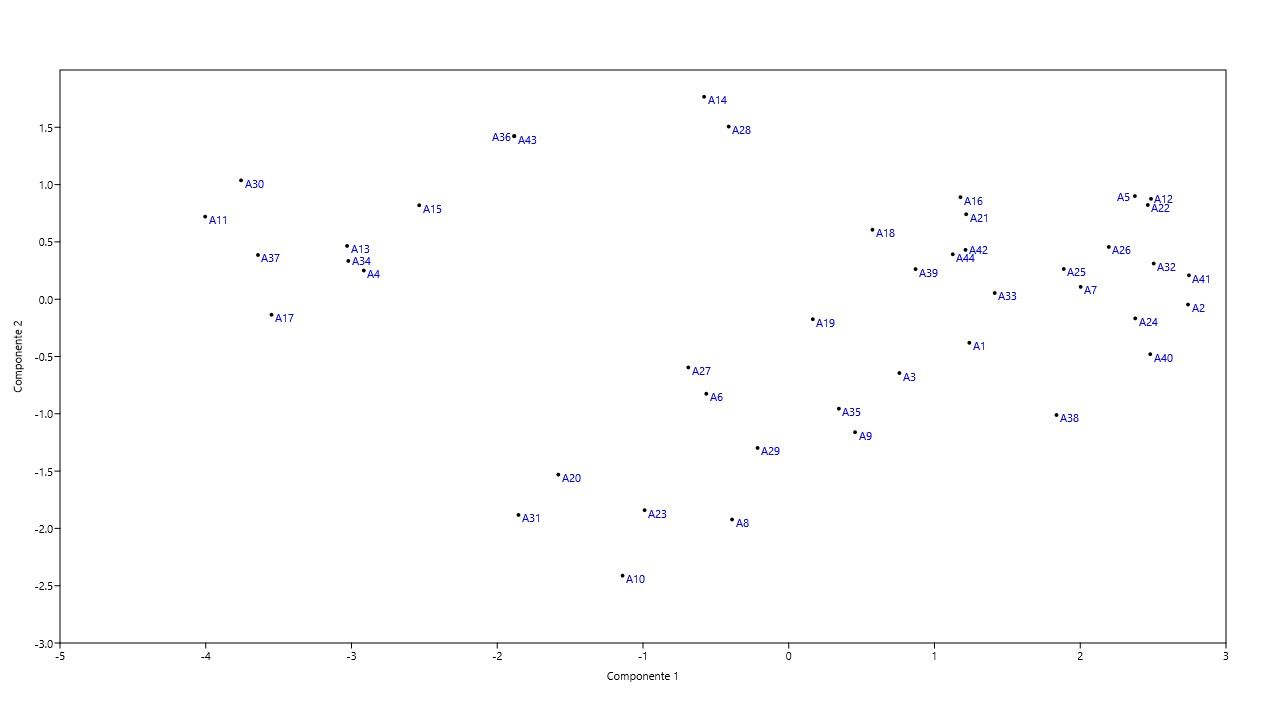
\includegraphics[width=1\textwidth]{figures/Grafico_C1_C2!.jpg}
        
\end{figure}
\begin{center}
    [Fuente:  Elaboración propia]
    \label{fig:Plano principal}
\end{center}


A la hora de realizar el análisis  de componentes principales con la herramienta \textbf{Real Statistics} en excel, se obtiene un resumen por cada componente, indicando así los porcentajes de datos que estos representan dentro de conjunto total estudiado, en este caso en el cuadro \ref{tab:Resumen}, se puede apreciar como el primer componente representa un 61.13\% y el segundo un 14.19\%, siendo así que entre las dos pueden representar un 75.32\% de todos los datos del conjunto, por lo cual a pesar de perder 24.68\%, la mejor opción para ver los datos es tomar los primeros 2 componentes que son los que mejor representan el conjunto.

\begin{table}[H]
\centering
\begin{tabular}{|c|c|c|c|}
\hline
\textbf{Comp. principal} & \textbf{Valor propio} & \textbf{Varianza} & \textbf{Acumulado} \\ \hline
\textbf{1}               & 4.27888             & 61.13\%           & 61,13\%            \\ \hline
\textbf{2}               & 0.993184            & 14.19\%           & 75,32\%            \\ \hline
\textbf{3}               & 0.620359            & 8.86\%            & 84,18\%            \\ \hline
\textbf{4}               & 0.44753             & 6.39\%            & 90,57\%            \\ \hline
\textbf{5}               & 0.337093            & 4.82\%            & 95,39\%            \\ \hline
\textbf{6}               & 0.186414            & 2.66\%            & 98,05\%            \\ \hline
\textbf{7}               & 0.136545            & 1.95\%            & 100\%              \\ \hline
\end{tabular}
\caption{Resumen de la matriz de correlación}
\label{tab:Resumen}
\end{table}


El gráfico de sedimentación lo generamos a partir de los datos de la tabla \ref{tab:Resumen}, el cual es usado para ver cuáles son los valores más representativos de los componentes, en este caso como se puede apreciar en el cuadro \ref{fig:Sedimentacion}, se deben tomar los componentes que se encuentren antes de la curva, que es este caso son los componentes 1 y 2, y descartar aquellos donde la gráfica toma una tendencia más recta como se ven en los componentes del 3 al 7.


\begin{figure}[H]
        \centering
        \caption{Gráfico de sedimentación}
        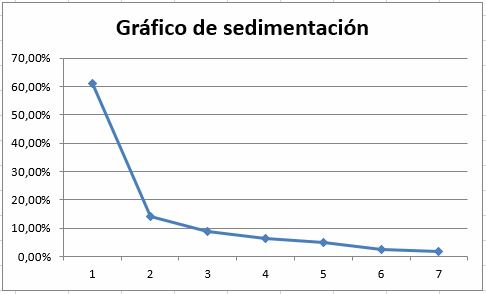
\includegraphics[width=0.8\textwidth]{figures/GraficoDeSedimantacion.JPG}
        \label{fig:Sedimentacion}
\end{figure}
\begin{center}
    [Fuente:  Elaboración propia]
\end{center}


De forma de introducción para el análisis de las distintas representaciones de los componentes resultantes. Según lo mostrado en la figura \ref{fig:Plano principal} la cual es el plano principal de los datos de la matriz original, tiene como objetivo una mayor visibilidad de los datos en el plano cartesiano. Este plano principal se proyectará por medio los componentes principales en tan solo dos dimensiones, ya sean los siguientes componentes:


\begin{itemize}
    \item \textbf{Componente 1} representa la evaluación de la tarea 1
    \item \textbf{Componente 2} representa la evaluación de la tarea 2
    \item \textbf{Componente 3} representa la evaluación de la tarea 3
    \item \textbf{Componente 4} representa la evaluación de la exposición
    \item \textbf{Componente 5} representa la evaluación el parcial 1
    \item \textbf{Componente 6} representa la evaluación el parcial 2 
    \item \textbf{Componente 7} representa la evaluación el proyecto
\end{itemize}


Lo que hace el análisis de componentes es buscar el mejor ángulo para presentar todos los datos de la tabla original \ref{tab:notas}. Cada componente representa un ángulo distinto en el que se obtiene los datos según el algoritmo propuesto en la sección \ref{ch:rutina}. 


A continuación podremos observar los componentes principales.
En la gráfica número uno que relaciona el componente 1 y 2, se pueden observar dos conglomerados en donde sé perciben conjuntos de datos relativamente cerca. Lo cual nos indica una mayor relación o una mayor porcentaje de representación, en este caso sería 75.32\% 

En cambio la figura 2 del componente 1 y 3 son más dispersos, lo cual es lógico, ya que ambos suman 69.99\%, lo cual se pierde un 30.1 \%  de datos.

\begin{figure}[H]
 \centering
  \caption{Representación de componentes 1, 2 y 3. }
  \subfloat[Comp. 1 y comp. 2]{

    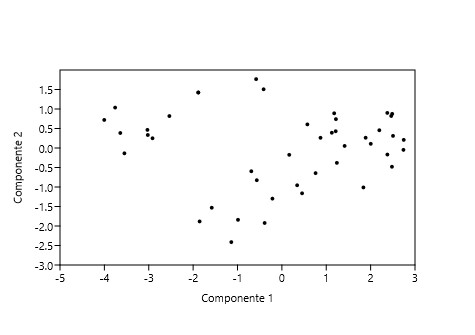
\includegraphics[width=0.5\textwidth]{figures/C1_C2.jpg}}
  \subfloat[Comp. 1 y comp. 3]{

    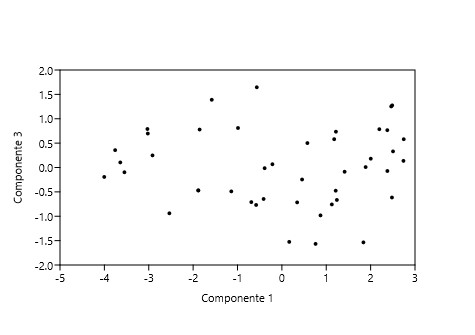
\includegraphics[width=0.5\textwidth]{figures/C1_C3.jpg}}
   

 \begin{center}
    [Fuente:  Elaboración propia]
\end{center}
\end{figure}


En la siguiente imagen se pueden observar que en la primera imagen se observan con la misma lógica anterior que se encuentran datos dispersos los cual representa el 67.52\% de datos en cambio la segunda imagen representa 23.05\%. 

Se puede entender claramente  que el componente 1 y 2 son las variables con mayor datos de representación de los datos originales. Conforme se va comparando con diferentes componentes a partir del 1 y 2, se puede apreciar que disminuye la cantidad de porcentajes de datos principales. 

\begin{figure}[H]
 \centering
  \caption{Representación de componentes 1, 2, 3 y 4. }
  \subfloat[Comp. 1 y comp. 4]{

    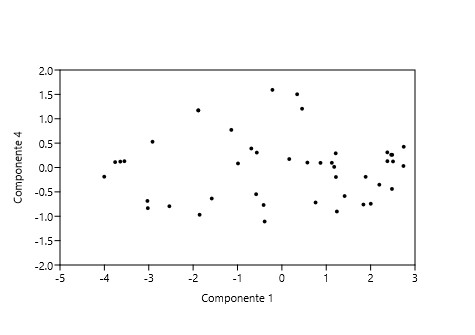
\includegraphics[width=0.5\textwidth]{figures/C1_C4.jpg}}
  \subfloat[Comp. 2 y comp. 3]{

    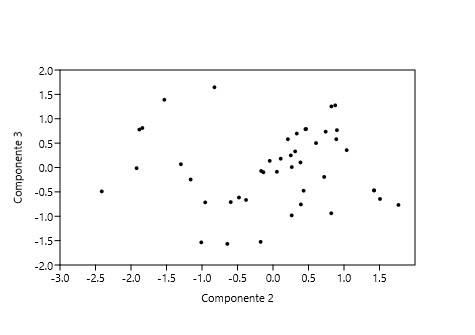
\includegraphics[width=0.5\textwidth]{figures/C2_C3.jpg}}
   
 \label{f:animales}
 \begin{center}
    [Fuente:  Elaboración propia]
\end{center}
\end{figure}



\begin{figure}[H]
 \centering
  \caption{Representación de componentes 2, 3 y 4. }
  \subfloat[Comp. 2 y comp. 4]{

    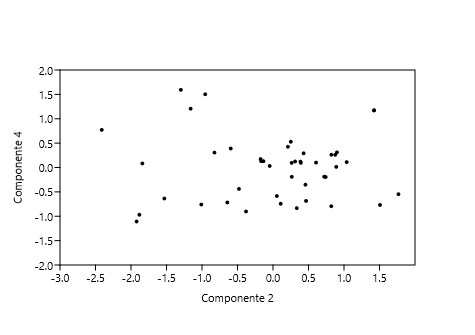
\includegraphics[width=0.5\textwidth]{figures/C2_C4.jpg}}
  \subfloat[Comp. 3 y comp. 4]{

    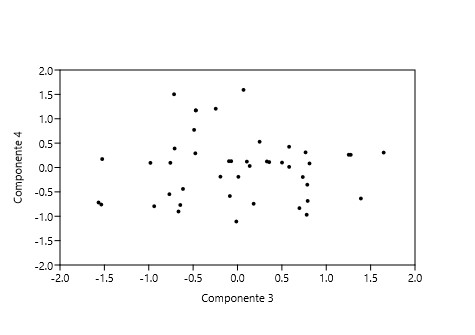
\includegraphics[width=0.5\textwidth]{figures/C3_C4.jpg}}
   

 \begin{center}
    [Fuente:  Elaboración propia]
\end{center}
\end{figure}

En las tablas anteriores se evalúan los componentes de 4 y 2 representan el 20.58\% de los datos, lo que seria nuestra columna de exposiciones y tarea 2 respectivamente, se puede apreciar que el componente 4 y el componente 2 representan muy poca de la información de los datos dando como 79.42\% de perdida de información. 

Muy parecido al gráfico adjunto, donde se evalúa el componente 4, el componente 4 con respecto al componente 3 que representan un 15.26\% de los datos, con el detalle donde ambos componentes ya presenta un agotamiento de la información en sus resultados, de los cuales se están perdiendo un 84.74\% de los datos.  


\begin{figure}[H]
        \centering
        \caption{Círculo de correlación}
        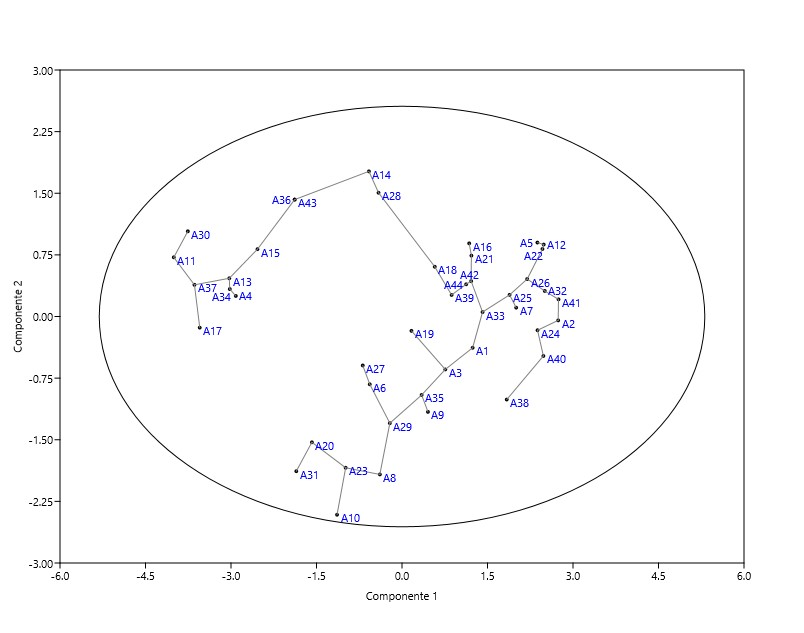
\includegraphics[width=0.8\textwidth]{figures/CirculoCorrelacion.jpg}
        
\end{figure}
\begin{center}
    [Fuente:  Elaboración propia]
\end{center}

Como se puede observar en el gráfico anterior de correlaciones, donde se evalúan los componentes 2 con respecto al componente 1, que representan un 75.32\% de los datos, los puntos que están más cerca del borde del círculo están mejor representados que los que están un poco más lejos, además de ser los componentes con mayor información, se pueden observar las relaciones entre componentes y el conglomerado entre puntos.  



